\documentclass[10pt]{article}
\usepackage[polish]{babel}
\usepackage[utf8]{inputenc}
\usepackage[T1]{fontenc}
\usepackage{amsmath}
\usepackage{amsfonts}
\usepackage{amssymb}
\usepackage[version=4]{mhchem}
\usepackage{stmaryrd}
\usepackage{graphicx}
\usepackage[export]{adjustbox}
\graphicspath{ {./images/} }

%New command to display footnote whose markers will always be hidden
\let\svthefootnote\thefootnote
\newcommand\blfootnotetext[1]{%
  \let\thefootnote\relax\footnote{#1}%
  \addtocounter{footnote}{-1}%
  \let\thefootnote\svthefootnote%
}

%Overriding the \footnotetext command to hide the marker if its value is `0`
\let\svfootnotetext\footnotetext
\renewcommand\footnotetext[2][?]{%
  \if\relax#1\relax%
    \ifnum\value{footnote}=0\blfootnotetext{#2}\else\svfootnotetext{#2}\fi%
  \else%
    \if?#1\ifnum\value{footnote}=0\blfootnotetext{#2}\else\svfootnotetext{#2}\fi%
    \else\svfootnotetext[#1]{#2}\fi%
  \fi
}

\DeclareUnicodeCharacter{00D7}{\ifmmode\times\else{$\times$}\fi}

\begin{document}
\section*{CENTRALNA \\
 KOMISJA \\
 EGZAMINACYJNA}
\begin{center}
\begin{tabular}{|l|l|}
\hline
Rodzaj dokumentu: & \begin{tabular}{l}
Zasady oceniania rozwiązań \\
zadań \\
\end{tabular} \\
\hline
Egzamin: & Egzamin maturalny \\
\hline
Przedmiot: & Matematyka \\
\hline
Poziom: & \begin{tabular}{l}
EMZiOM podstawowy \\
EMAP-P0-100-2105 (wersje arkusza: A i B), \\
\hline
Formy arkusza: \\
\hline
\end{tabular} \\
\hline
\begin{tabular}{l}
EMAP-P0-400-2105, EMAP-P0-600-2105, \\
EMAP-2105, EMAP-P0-300-2105, \\
EMAP-P0-700-2105, EMAP-P0-Q00-2105 \\
\end{tabular} &  \\
\hline
Termin egzaminu: & 5 maja 2021 r. \\
\hline
\begin{tabular}{l}
Data publikacji \\
dokumentu: \\
\end{tabular} & 21 czerwca 2021 r. \\
\hline
\end{tabular}
\end{center}

\section*{Uwaga:}
Gdy wymaganie egzaminacyjne dotyczy treści z III etapu edukacyjnego - dopisano „G".

\section*{ZADANIA ZAMKNIETE}
\section*{Zadanie 1. (0-1)}
\begin{center}
\begin{tabular}{|l|l|}
\hline
\multicolumn{2}{|c|}{${\text { Wymagania egzaminacyjne } \text { 2021 }^{1}}^{|c|}$ Wymaganie ogólne} \\
\multicolumn{1}{|c|}{Wymaganie szczegółowe $^{|c|}$} &  \\
\hline
II. Wykorzystanie i interpretowanie & Zdający: \\
reprezentacji. & 1.4) oblicza potęgi o wykładnikach \\
 & wymiernych i stosuje prawa działań na \\
 & potęgach o wykładnikach wymiernych. \\
\hline
\end{tabular}
\end{center}

\section*{Zasady oceniania}
1 pkt - odpowiedź poprawna.\\
0 pkt - odpowiedź niepoprawna albo brak odpowiedzi.

\section*{Rozwiązanie}
Wersja A: B\\
Wersja B: D\\
Zadanie 2. (0-1)

\begin{center}
\begin{tabular}{|l|l|}
\hline
\multicolumn{2}{|c|}{Wymagania egzaminacyjne 2021} \\
\hline
\multicolumn{1}{|c|}{Wymaganie ogólne} & \multicolumn{1}{|c|}{Wymaganie szczegółowe} \\
\hline
\begin{tabular}{ll}
\multicolumn{1}{|c|}{II. Wykorzystanie i interpretowanie} & Zdający: \\
reprezentacji. & 1.8) wykonuje obliczenia procentowe [...]. \\
\hline
\end{tabular} &  \\
\hline
\end{tabular}
\end{center}

\section*{Zasady oceniania}
1 pkt - odpowiedź poprawna.\\
0 pkt - odpowiedź niepoprawna albo brak odpowiedzi.

\section*{Rozwiązanie}
Wersja A: B\\
Wersja B: C

\footnotetext{${ }^{1}$ Załącznik nr 2 do rozporządzenia Ministra Edukacji Narodowej z dnia 20 marca 2020 r. w sprawie szczególnych rozwiązań w okresie czasowego ograniczenia funkcjonowania jednostek systemu oświaty w związku z zapobieganiem, przeciwdziałaniem i zwalczaniem COVID-19 (Dz.U. poz. 493, z późn. zm.).
}Zadanie 3. (0-1)

\begin{center}
\begin{tabular}{|l|l|}
\hline
\multicolumn{2}{|c|}{Wymagania egzaminacyjne 2021} \\
\hline
\multicolumn{1}{|c|}{Wymaganie ogólne} & \multicolumn{1}{c|}{Wymaganie szczegółowe} \\
\hline
II. Wykorzystanie i interpretowanie & Zdający: \\
reprezentacji. & \begin{tabular}{l}
1.7) posługuje się pojęciem przedziału \\
liczbowego, zaznacza przedziały na osi \\
liczbowej. \\
\end{tabular} \\
\hline
\end{tabular}
\end{center}

\section*{Zasady oceniania}
1 pkt - odpowiedź poprawna.\\
0 pkt - odpowiedź niepoprawna albo brak odpowiedzi.

\section*{Rozwiązanie}
Wersja A: A\\
Wersja B: B\\
Zadanie 4. (0-1)

\begin{center}
\begin{tabular}{|l|l|}
\hline
\multicolumn{2}{|c|}{Wymagania egzaminacyjne 2021} \\
\hline
\multicolumn{1}{|c|}{Wymaganie ogólne} & \multicolumn{1}{c|}{Wymaganie szczegółowe} \\
\hline
\begin{tabular}{ll}
II. Wykorzystanie i interpretowanie &  \\
reprezentacji. & Zdający: \\
 & \begin{tabular}{l}
1.6) wykorzystuje definicję logarytmu \\
i stosuje w obliczeniach wzory na logarytm \\
iloczynu [...] i logarytm potęgi o wykładniku \\
naturalnym. \\
\end{tabular} \\
\hline
\end{tabular} &  \\
\hline
\end{tabular}
\end{center}

\section*{Zasady oceniania}
1 pkt - odpowiedź poprawna.\\
0 pkt - odpowiedź niepoprawna albo brak odpowiedzi.

\section*{Rozwiązanie}
Wersja A: C\\
Wersja B: A\\
Zadanie 5. (0-1)

\begin{center}
\begin{tabular}{|l|l|}
\hline
\multicolumn{2}{|c|}{Wymagania egzaminacyjne 2021} \\
\hline
\multicolumn{1}{|c|}{Wymaganie ogólne} & \multicolumn{1}{c|}{Wymaganie szczegółowe} \\
\hline
I. Wykorzystanie i tworzenie informacji. & \begin{tabular}{l}
Zdający: \\
 \\
 \\
 \\
 \\
 \\
 \\
 \\
 \\
 \\
 \\
w różžych postaciach (np. ułamka \\
zwykłego, ułamka dziesiętnego \\
okresowego [...]). \\
\end{tabular} \\
\hline
\end{tabular}
\end{center}

\section*{Zasady oceniania}
1 pkt - odpowiedź poprawna.\\
0 pkt - odpowiedź niepoprawna albo brak odpowiedzi.

\section*{Rozwiązanie}
Wersja A: D\\
Wersja B: B\\
Zadanie 6. (0-1)

\begin{center}
\begin{tabular}{|l|l|}
\hline
\multicolumn{2}{|c|}{Wymagania egzaminacyjne 2021} \\
\hline
\multicolumn{1}{|c|}{Wymaganie ogólne} & \multicolumn{1}{c|}{Wymaganie szczegółowe} \\
\hline
II. Wykorzystanie i interpretowanie & \begin{tabular}{l}
Zdający: \\
reprezentacji. \\
\end{tabular} \\
\hline
\end{tabular}
\end{center}

\section*{Zasady oceniania}
1 pkt - odpowiedź poprawna.\\
0 pkt - odpowiedź niepoprawna albo brak odpowiedzi.

\section*{Rozwiązanie}
Wersja A: B\\
Wersja B: C

\section*{Zadanie 7. (0-1)}
\begin{center}
\begin{tabular}{|c|c|}
\hline
\multicolumn{2}{|c|}{Wymagania egzaminacyjne 2021} \\
\hline
Wymaganie ogólne & Wymaganie szczegółowe \\
\hline
I. Wykorzystanie i tworzenie informacji. & \begin{tabular}{l}
Zdający: \\
4.3) odczytuje z wykresu własności funkcji (dziedzinę, zbiór wartości, miejsca zerowe [...]). \\
\end{tabular} \\
\hline
\end{tabular}
\end{center}

\section*{Zasady oceniania}
1 pkt - odpowiedź poprawna.\\
0 pkt - odpowiedź niepoprawna albo brak odpowiedzi.

\section*{Rozwiązanie}
Wersja A: A\\
Wersja B: D\\
Zadanie 8. (0-1)

\begin{center}
\begin{tabular}{|l|l|}
\hline
\multicolumn{2}{|c|}{Wymagania egzaminacyjne 2021} \\
\hline
\multicolumn{1}{|c|}{Wymaganie ogólne} & \multicolumn{1}{c|}{Wymaganie szczegółowe} \\
\hline
II. Wykorzystanie i interpretowanie & \begin{tabular}{l}
Zdający: \\
reprezentacji. \\
\end{tabular} \\
\begin{tabular}{l}
3.2) wykorzystuje interpretacjé \\
geometryczną układu równań pierwszego \\
stopnia z dwiema niewiadomymi. \\
\end{tabular} &  \\
\hline
\end{tabular}
\end{center}

\section*{Zasady oceniania}
1 pkt - odpowiedź poprawna.\\
0 pkt - odpowiedź niepoprawna albo brak odpowiedzi.

\section*{Rozwiązanie}
Wersja A: A\\
Wersja B: C\\
Zadanie 9. (0-1)

\begin{center}
\begin{tabular}{|l|l|}
\hline
\multicolumn{2}{|c|}{Wymagania egzaminacyjne 2021} \\
\hline
\multicolumn{1}{|c|}{Wymaganie ogólne} & \multicolumn{1}{c|}{Wymaganie szczegółowe} \\
\hline
\multicolumn{1}{|c|}{II. Wykorzystanie i interpretowanie} & Zdający: \\
reprezentacji. & 4.7) interpretuje współczynniki \\
 & występujące we wzorze funkcji liniowej. \\
\hline
\end{tabular}
\end{center}

\section*{Zasady oceniania}
1 pkt - odpowiedź poprawna.\\
0 pkt - odpowiedź niepoprawna albo brak odpowiedzi.

\section*{Rozwiązanie}
Wersja A: D\\
Wersja B: A

\section*{Zadanie 10. (0-1)}
\begin{center}
\begin{tabular}{|l|l|}
\hline
\multicolumn{2}{|c|}{Wymagania egzaminacyjne 2021} \\
\hline
\multicolumn{1}{|c|}{Wymaganie ogólne} & \multicolumn{1}{c|}{Wymagania szczegółowe} \\
\hline
II. Wykorzystanie i interpretowanie & Zdający: \\
reprezentacji. & 2.1) używa wzorów skróconego mnożenia \\
 & na $(a \pm b)^{2}$ oraz $a^{2}-b^{2} ;$ \\
 & 4.2) oblicza ze wzoru wartość funkcji dla \\
 & danego argumentu $[\ldots]$. \\
\hline
\end{tabular}
\end{center}

\section*{Zasady oceniania}
1 pkt - odpowiedź poprawna.\\
0 pkt - odpowiedź niepoprawna albo brak odpowiedzi.

\section*{Rozwiązanie}
Wersja A: B\\
Wersja B: C\\
Zadanie 11. (0-1)

\begin{center}
\begin{tabular}{|l|l|}
\hline
\multicolumn{2}{|c|}{Wymagania egzaminacyjne 2021} \\
\hline
\multicolumn{1}{|c|}{Wymaganie ogólne} & \multicolumn{1}{c|}{Wymaganie szczegółowe} \\
\hline
II. Wykorzystanie i interpretowanie & \begin{tabular}{l}
Zdający: \\
reprezentacji. \\
\end{tabular} \\
 & \begin{tabular}{l}
4.2) oblicza ze wzoru wartość funkcji dla \\
danego argumentu [...]. \\
\end{tabular} \\
\hline
\end{tabular}
\end{center}

\section*{Zasady oceniania}
1 pkt - odpowiedź poprawna.\\
0 pkt - odpowiedź niepoprawna albo brak odpowiedzi.

\section*{Rozwiązanie}
Wersja A: C\\
Wersja B: B\\
Zadanie 12. (0-1)

\begin{center}
\begin{tabular}{|l|l|}
\hline
\multicolumn{2}{|c|}{Wymagania egzaminacyjne 2021} \\
\hline
\multicolumn{1}{|c|}{Wymaganie ogólne} & \multicolumn{1}{c|}{Wymaganie szczegółowe} \\
\hline
II. Wykorzystanie i interpretowanie & Zdający: \\
reprezentacji. & 4.3) odczytuje z wykresu własności funkcji \\
 & ([...] maksymalne przedziały, w których \\
funkcja maleje, rośnie, ma stały znak [...]). &  \\
\hline
\end{tabular}
\end{center}

\section*{Zasady oceniania}
1 pkt - odpowiedź poprawna.\\
0 pkt - odpowiedź niepoprawna albo brak odpowiedzi.

\section*{Rozwiązanie}
Wersja A: A\\
Wersja B: D\\
Zadanie 13. (0-1)

\begin{center}
\begin{tabular}{|l|l|}
\hline
\multicolumn{2}{|c|}{Wymagania egzaminacyjne 2021} \\
\hline
\multicolumn{1}{|c|}{Wymaganie ogólne} & \multicolumn{1}{c|}{Wymaganie szczegółowe} \\
\hline
\multicolumn{1}{|c|}{II. Wykorzystanie i interpretowanie} & Zdający: \\
reprezentacji. & \begin{tabular}{l}
5.4) stosuje wzór na $n$-ty wyraz [...] ciągu \\
geometrycznego. \\
\end{tabular} \\
\hline
\end{tabular}
\end{center}

\section*{Zasady oceniania}
1 pkt - odpowiedź poprawna.\\
0 pkt - odpowiedź niepoprawna albo brak odpowiedzi.

\section*{Rozwiązanie}
Wersja A: D\\
Wersja B: B\\
Zadanie 14. (0-1)

\begin{center}
\begin{tabular}{|l|l|}
\hline
\multicolumn{2}{|c|}{Wymagania egzaminacyjne 2021} \\
\hline
\multicolumn{1}{|c|}{Wymaganie ogólne} & \multicolumn{1}{c|}{Wymaganie szczegółowe} \\
\hline
III. Modelowanie matematyczne. & Zdający: \\
 & \begin{tabular}{l}
5.1) wyznacza wyrazy ciągu określonego \\
 \\
 \\
\end{tabular} wzorem ogólnym. \\
\hline
\end{tabular}
\end{center}

\section*{Zasady oceniania}
1 pkt - odpowiedź poprawna.\\
0 pkt - odpowiedź niepoprawna albo brak odpowiedzi.

\section*{Rozwiązanie}
Wersja A: D\\
Wersja B: A\\
Zadanie 15. (0-1)

\begin{center}
\begin{tabular}{|l|l|}
\hline
\multicolumn{2}{|c|}{Wymagania egzaminacyjne 2021} \\
\hline
\multicolumn{1}{|c|}{Wymaganie ogólne} & \multicolumn{1}{c|}{Wymaganie szczegółowe} \\
\hline
II. Wykorzystanie i interpretowanie & \begin{tabular}{l}
Zdający: \\
reprezentacji. \\
\end{tabular} \\
 & \begin{tabular}{l}
5.3) stosuje wzór na $n$-ty wyraz i na sumę \\
$n$ początkowych wyrazów ciągu \\
arytmetycznego. \\
\end{tabular} \\
\hline
\end{tabular}
\end{center}

\section*{Zasady oceniania}
1 pkt - odpowiedź poprawna.\\
0 pkt - odpowiedź niepoprawna albo brak odpowiedzi.

\section*{Rozwiązanie}
Wersja A: B\\
Wersja B: D\\
Zadanie 16. (0-1)

\begin{center}
\begin{tabular}{|l|l|}
\hline
\multicolumn{2}{|c|}{Wymagania egzaminacyjne 2021} \\
\hline
\multicolumn{1}{|c|}{Wymaganie ogólne} & \multicolumn{1}{c|}{Wymaganie szczegółowe} \\
\hline
II. Wykorzystanie i interpretowanie & \begin{tabular}{l}
Zdający: \\
reprezentacji. \\
\end{tabular} \\
 & \begin{tabular}{l}
6.3) stosuje proste zależności między \\
funkcjami trygonometrycznymi [..]. \\
\end{tabular} \\
\hline
\end{tabular}
\end{center}

\section*{Zasady oceniania}
1 pkt - odpowiedź poprawna.\\
0 pkt - odpowiedź niepoprawna albo brak odpowiedzi.

\section*{Rozwiązanie}
Wersja A: B\\
Wersja B: A\\
Zadanie 17. (0-1)

\begin{center}
\begin{tabular}{|l|l|}
\hline
\multicolumn{2}{|c|}{Wymagania egzaminacyjne 2021} \\
\hline
\multicolumn{1}{|c|}{Wymaganie ogólne} & \multicolumn{1}{c|}{Wymaganie szczegółowe} \\
\hline
IV. Użycie i tworzenie strategii. & \begin{tabular}{l}
Zdający: \\
 \\
 \\
 \\
 \\
\hline
\end{tabular} o.2) korzysta z własności stycznej do \\
okręgu. &  \\
\end{tabular}
\end{center}

\section*{Zasady oceniania}
1 pkt - odpowiedź poprawna.\\
0 pkt - odpowiedź niepoprawna albo brak odpowiedzi.

\section*{Rozwiązanie}
Wersja A: C\\
Wersja B: B\\
Zadanie 18. (0-1)

\begin{center}
\begin{tabular}{|l|l|}
\hline
\multicolumn{2}{|c|}{Wymagania egzaminacyjne 2021} \\
\hline
\multicolumn{1}{|c|}{Wymaganie ogólne} & \multicolumn{1}{|c|}{Wymaganie szczegółowe} \\
\hline
IV. Użycie i tworzenie strategii. & \begin{tabular}{l}
Zdający: \\
 \\
 \\
 \\
 \\
 \\
 \\
 \\
tryg konzysta z własności funkcji \\
obliczeniach geometrycznych [...]. \\
\hline
\end{tabular} \\
\hline
\end{tabular}
\end{center}

\section*{Zasady oceniania}
1 pkt - odpowiedź poprawna.\\
0 pkt - odpowiedź niepoprawna albo brak odpowiedzi.

\section*{Rozwiązanie}
Wersja A: D\\
Wersja B: D\\
Zadanie 19. (0-1)

\begin{center}
\begin{tabular}{|l|l|}
\hline
\multicolumn{2}{|c|}{Wymagania egzaminacyjne 2021} \\
\hline
\multicolumn{1}{|c|}{Wymaganie ogólne} & \multicolumn{1}{c|}{Wymaganie szczegółowe} \\
\hline
II. Wykorzystanie i interpretowanie & Zdający: \\
reprezentacji. & G10.9) oblicza pola i obwody trójkątów \\
 & $[\ldots .]$. \\
\hline
\end{tabular}
\end{center}

\section*{Zasady oceniania}
1 pkt - odpowiedź poprawna.\\
0 pkt - odpowiedź niepoprawna albo brak odpowiedzi.

\section*{Rozwiązanie}
Wersja A: A\\
Wersja B: C\\
Zadanie 20. (0-1)

\begin{center}
\begin{tabular}{|l|l|}
\hline
\multicolumn{2}{|c|}{Wymagania egzaminacyjne 2021} \\
\hline
\multicolumn{1}{|c|}{Wymaganie ogólne} & \multicolumn{1}{c|}{Wymaganie szczegółowe} \\
\hline
\begin{tabular}{ll}
II. Wykorzystanie i interpretowanie &  \\
reprezentacji. & Zdający: \\
G10.7) stosuje twierdzenie Pitagorasa. &  \\
\hline
\end{tabular} &  \\
\hline
\end{tabular}
\end{center}

\section*{Zasady oceniania}
1 pkt - odpowiedź poprawna.\\
0 pkt - odpowiedź niepoprawna albo brak odpowiedzi.

\section*{Rozwiązanie}
Wersja A: A\\
Wersja B: B\\
Zadanie 21. (0-1)

\begin{center}
\begin{tabular}{|l|l|}
\hline
\multicolumn{2}{|c|}{Wymagania egzaminacyjne 2021} \\
\hline
\multicolumn{1}{|c|}{Wymaganie ogólne} & \multicolumn{1}{c|}{Wymaganie szczegółowe} \\
\hline
\multicolumn{1}{|c|}{II. Wykorzystanie i interpretowanie} & Zdający: \\
reprezentacji. & \begin{tabular}{l}
7.1) stosuje zależności między kątem \\
środkowym i kątem wpisanym. \\
\end{tabular} \\
\hline
\end{tabular}
\end{center}

\section*{Zasady oceniania}
1 pkt - odpowiedź poprawna.\\
0 pkt - odpowiedź niepoprawna albo brak odpowiedzi.

\section*{Rozwiązanie}
Wersja A: D\\
Wersja B: B\\
Zadanie 22. (0-1)

\begin{center}
\begin{tabular}{|l|l|}
\hline
\multicolumn{2}{|c|}{Wymagania egzaminacyjne 2021} \\
\hline
\multicolumn{1}{|c|}{Wymaganie ogólne} & \multicolumn{1}{c|}{Wymaganie szczegółowe} \\
\hline
\multicolumn{1}{|c|}{II. Wykorzystanie i interpretowanie} & Zdający: \\
reprezentacji. & G10.8) korzysta z własności kątów \\
 & i przekąnych w prostokątach, \\
 & równoległobokach, rombach i w trapezach. \\
\hline
\end{tabular}
\end{center}

\section*{Zasady oceniania}
1 pkt - odpowiedź poprawna.\\
0 pkt - odpowiedź niepoprawna albo brak odpowiedzi.

\section*{Rozwiązanie}
Wersja A: B\\
Wersja B: C\\
Zadanie 23. (0-1)

\begin{center}
\begin{tabular}{|l|l|}
\hline
\multicolumn{2}{|c|}{Wymagania egzaminacyjne 2021} \\
\hline
\multicolumn{1}{|c|}{Wymaganie ogólne} & \multicolumn{1}{c|}{Wymaganie szczegółowe} \\
\hline
II. Wykorzystanie i interpretowanie & \begin{tabular}{l}
Zdający: \\
reprezentacji. \\
\end{tabular} \\
 & \begin{tabular}{l}
3.4) rozwiązuje równania kwadratowe \\
z jedną niewiadomą. \\
\end{tabular} \\
\hline
\end{tabular}
\end{center}

\section*{Zasady oceniania}
1 pkt - odpowiedź poprawna.\\
0 pkt - odpowiedź niepoprawna albo brak odpowiedzi.

\section*{Rozwiązanie}
Wersja A: B\\
Wersja B: B\\
Zadanie 24. (0-1)

\begin{center}
\begin{tabular}{|l|l|}
\hline
\multicolumn{2}{|c|}{Wymagania egzaminacyjne 2021} \\
\hline
\multicolumn{1}{|c|}{Wymaganie ogólne} & \multicolumn{1}{|c|}{Wymaganie szczegółowe} \\
\hline
III. Modelowanie matematyczne. & Zdający: \\
 & G10.6) oblicza pole koła [...]. \\
\hline
\end{tabular}
\end{center}

\section*{Zasady oceniania}
1 pkt - odpowiedź poprawna.\\
0 pkt - odpowiedź niepoprawna albo brak odpowiedzi.

\section*{Rozwiązanie}
Wersja A: C\\
Wersja B: D

\section*{Zadanie 25. (0-1)}
\begin{center}
\begin{tabular}{|l|l|}
\hline
\multicolumn{2}{|c|}{Wymagania egzaminacyjne 2021} \\
\hline
\multicolumn{1}{|c|}{Wymaganie ogólne} & \multicolumn{1}{c|}{Wymaganie szczegółowe} \\
\hline
IV. Użycie i tworzenie strategii. & Zdający: \\
 & 8.6) oblicza odległość dwóch punktów. \\
\hline
\end{tabular}
\end{center}

\section*{Zasady oceniania}
1 pkt - odpowiedź poprawna.\\
0 pkt - odpowiedź niepoprawna albo brak odpowiedzi.

\section*{Rozwiązanie}
Wersja A: B\\
Wersja B: D\\
Zadanie 26. (0-1)

\begin{center}
\begin{tabular}{|l|l|}
\hline
\multicolumn{2}{|c|}{Wymagania egzaminacyjne 2021} \\
\hline
\multicolumn{1}{|c|}{Wymaganie ogólne} & \multicolumn{1}{|c|}{Wymaganie szczegółowe} \\
\hline
III. Modelowanie matematyczne. & Zdający: \\
 & 10.2) oblicza prawdopodobieństwa \\
 & w prostych sytuacjach, stosując klasyczną \\
 & definicję prawdopodobieństwa. \\
\hline
\end{tabular}
\end{center}

\section*{Zasady oceniania}
1 pkt - odpowiedź poprawna.\\
0 pkt - odpowiedź niepoprawna albo brak odpowiedzi.

\section*{Rozwiązanie}
Wersja A: A\\
Wersja B: B\\
Zadanie 27. (0-1)

\begin{center}
\begin{tabular}{|l|l|}
\hline
\multicolumn{2}{|c|}{Wymagania egzaminacyjne 2021} \\
\hline
\multicolumn{1}{|c|}{Wymaganie ogólne} & \multicolumn{1}{c|}{Wymaganie szczegółowe} \\
\hline
III. Modelowanie matematyczne. & \begin{tabular}{l}
Zdający: \\
 \\
 \\
 \\
 \\
 \\
 \\
 \\
 \\
 \\
 \\
ko.1) zlicza obiekty w prostych sytuacjach \\
użycia wzorów kombinatorycznych, stosuje \\
regułę mnożenia i reguł̨ dodawania. \\
\end{tabular} \\
\hline
\end{tabular}
\end{center}

\section*{Zasady oceniania}
1 pkt - odpowiedź poprawna.\\
0 pkt - odpowiedź niepoprawna albo brak odpowiedzi.

\section*{Rozwiązanie}
Wersja A: B\\
Wersja B: C\\
Zadanie 28. (0-1)

\begin{center}
\begin{tabular}{|l|l|}
\hline
\multicolumn{2}{|c|}{Wymagania egzaminacyjne 2021} \\
\hline
\multicolumn{1}{|c|}{Wymaganie ogólne} & \multicolumn{1}{|c|}{Wymaganie szczegółowe} \\
\hline
III. Modelowanie matematyczne. & \begin{tabular}{l}
Zdajacy: \\
 \\
 \\
 \\
 \\
 \\
 \\
 \\
 \\
G9.3) wyznacza [...] medianę zestawu \\
danych. \\
\hline
\end{tabular} \\
\hline
\end{tabular}
\end{center}

\section*{Zasady oceniania}
1 pkt - odpowiedź poprawna.\\
0 pkt - odpowiedź niepoprawna albo brak odpowiedzi.

\section*{Rozwiązanie}
Wersja A: C\\
Wersja B: B

\section*{ZADANIA OTWARTE}
\begin{enumerate}
  \item Akceptowane są wszystkie rozwiązania merytorycznie poprawne i spełniające warunki zadania.
  \item Jeżeli zdający poprawnie rozwiąże zadanie i otrzyma poprawny wynik, lecz w końcowym zapisie przekształca ten wynik i popełnia przy tym błąd, to może uzyskać maksymalną liczbę punktów.
  \item Jeżeli zdający popełni błędy rachunkowe, które na żadnym etapie rozwiązania nie upraszczają i nie zmieniają danego zagadnienia, lecz stosuje poprawną metodę i konsekwentnie do popełnionych błędów rachunkowych rozwiązuje zadanie, to może otrzymać co najwyżej $(n-1)$ punktów (gdzie $n$ jest maksymalną możliwą do uzyskania liczbą punktów za dane zadanie).
\end{enumerate}

Zadanie 29. (0-2)

\begin{center}
\begin{tabular}{|l|l|}
\hline
\multicolumn{2}{|c|}{Wymagania egzaminacyjne 2021} \\
\hline
\multicolumn{1}{|c|}{Wymaganie ogólne} & \multicolumn{1}{c|}{Wymaganie szczegółowe} \\
\hline
\begin{tabular}{l}
II. Wykorzystanie i interpretowanie \\
reprezentacji. \\
\end{tabular} & \begin{tabular}{l}
Zdający: \\
 \\
\end{tabular} \\
\begin{tabular}{l}
3.5) rozwiązuje nierówności kwadratowe \\
z jedną niewiadomą. \\
\end{tabular} &  \\
\hline
\end{tabular}
\end{center}

\section*{Zasady oceniania}
Rozwiązanie nierówności kwadratowej składa się z dwóch etapów.\\
Pierwszy etap to wyznaczenie pierwiastków trójmianu kwadratowego $x^{2}-5 x-14$.\\
Drugi etap to zapisanie zbioru rozwiązań nierówności kwadratowej $x^{2}-5 x-14 \leq 0$.\\
$\qquad$\\
Zdający otrzymuje 1 p. gdy:

\begin{itemize}
  \item obliczy lub poda pierwiastki trójmianu kwadratowego $x^{2}-5 x-14$ : $x_{1}=-2$ oraz $x_{2}=7$\\
ALBO
  \item odczyta z wykresu funkcji $f(x)=x^{2}-5 x-14$ i zapisze miejsca zerowe $x_{1}=-2$ oraz $x_{2}=7$
\end{itemize}

\section*{Zdający otrzymuje}
 2 p. gdy spełni warunki określone w zasadach oceniania za 1 pkt oraz:\begin{itemize}
  \item poda zbiór rozwiązań nierówności: $\langle-2,7\rangle$ lub $x \in\langle-2,7\rangle$
\end{itemize}

ALBO

\begin{itemize}
  \item poda zbiór rozwiązań nierówności w postaci graficznej z poprawnie zaznaczonymi końcami przedziałów\\
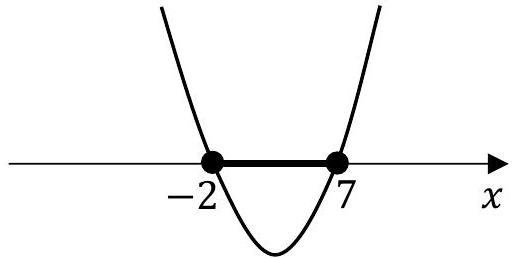
\includegraphics[max width=\textwidth, center]{2025_02_07_6828143ce1e2fe8e0865g-12}
\end{itemize}

\section*{Uwagi:}
\begin{enumerate}
  \item Jeżeli zdający, realizując pierwszy etap rozwiązania zadania, popełni błąd (ale otrzyma dwa różne pierwiastki) i konsekwentnie do popełnionego błędu zapisze zbiór rozwiązań nierówności, to otrzymuje 1 punkt za całe rozwiązanie.
  \item Jeżeli zdający wyznacza pierwiastki trójmianu kwadratowego w przypadku, gdy błędnie obliczony przez zdającego wyróżnik $\Delta$ jest ujemny, to otrzymuje $\mathbf{0}$ punktów za całe rozwiązanie.
  \item Jeżeli zdający, rozpoczynając realizację pierwszego etapu rozwiązania, rozpatruje inny niż podany w zadaniu trójmian kwadratowy i obliczy/poda pierwiastki tego rozpatrywanego trójmianu, to oznacza, że nie podjął realizacji 1. etapu rozwiązania i w konsekwencji otrzymuje 0 punktów za całe rozwiązanie.
  \item Akceptujemy zapisanie pierwiastków trójmianu w postaci $a+b \sqrt{c}$, gdzie $a, b, c$ są liczbami wymiernymi.
\end{enumerate}

\section*{Kryteria uwzględniające specyficzne trudności w uczeniu się matematyki}
Jeśli zdający pomyli porządek liczb na osi liczbowej, np. zapisze zbiór rozwiązań nierówności w postaci $\langle 7,-2\rangle$, to przyznajemy 2 punkty.

\section*{Przykładowe pełne rozwiązanie}
\section*{Pierwszy etap rozwiązania}
Zapisujemy nierówność w postaci $x^{2}-5 x-14 \leq 0$ i obliczamy pierwiastki trójmianu $x^{2}-5 x-14$.\\
Obliczamy wyróżnik tego trójmianu: $\Delta=81$ i stąd $x_{1}=-2$ oraz $x_{2}=7$.\\
ALBO

Stosujemy wzory Viète'a:\\
$x_{1} \cdot x_{2}=-14$ oraz $x_{1}+x_{2}=5$, stąd $x_{1}=-2$ oraz $x_{2}=7$.\\
ALBO

Podajemy je bezpośrednio, zapisując pierwiastki trójmianu lub zaznaczając je na wykresie:\\
$x_{1}=-2$ oraz $x_{2}=7$.

\section*{Drugi etap rozwiązania}
Podajemy zbiór rozwiązań nierówności: $\langle-2,7\rangle$ lub $x \in\langle-2,7\rangle$ lub zaznaczamy zbiór rozwiązań na osi liczbowej\\
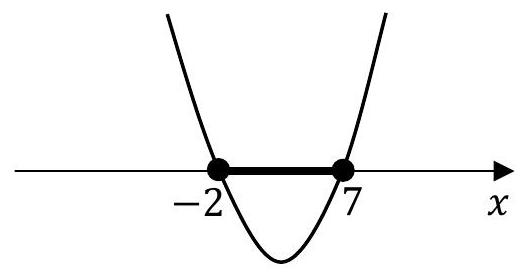
\includegraphics[max width=\textwidth, center]{2025_02_07_6828143ce1e2fe8e0865g-13}

Zadanie 30. (0-2)

\begin{center}
\begin{tabular}{|l|l|}
\hline
\multicolumn{2}{|c|}{Wymagania egzaminacyjne 2021} \\
\hline
\multicolumn{1}{|c|}{Wymaganie ogólne} & \multicolumn{1}{c|}{Wymagania szczegółowe} \\
\hline
V. Rozumowanie i argumentacja. & Zdający: \\
 & G6.4) dodaje i odejmuje sumy \\
 & algebraiczne; \\
 & G6.5) mnoży jednomiany, mnoży sumę \\
 & algebraiczną przez jednomian oraz, \\
 & w nietrudnych przypadkach, mnoży sumy \\
 & algebraiczne. \\
\hline
\end{tabular}
\end{center}

\section*{Zasady oceniania}
\section*{Zdający otrzymuje 1 p. \\
 gdy: \\
 - przekształci nierówność $\frac{a}{b}<\frac{a+c}{b+c}$ do postaci równoważnej, z której można przeprowadzić bezpośrednie wnioskowanie o prawdziwości tezy,}
np. 1) $\frac{c(a-b)}{b(b+c)}<0$ lub 2) $c(a-b)<0$ lub 3) $c a<c b$ lub 4) $\frac{a-b}{b}<\frac{a-b}{b+c}$\\
ALBO

\begin{itemize}
  \item przekształci nierówność $a<b$ do postaci równoważnej $a(b+c)<b(a+c)$
\end{itemize}

ALBO

\begin{itemize}
  \item przeprowadzając dowód nie wprost, przekształci nierówność $\frac{a}{b} \geq \frac{a+c}{b+c}$ (która jest zaprzeczeniem tezy) do postaci $a c \geq b c$
\end{itemize}

\section*{Zdający otrzymuje}
gdy przeprowadzi pełne rozumowanie - zdający musi spełnić warunki określone w zasadach oceniania za 1 punkt oraz:

\begin{itemize}
  \item wykorzystać założenie $a<b$ w sytuacjach 1), 2), 3) określonych w pierwszym punktorze zasad oceniania za 1 punkt\\
ALBO
  \item wykorzystać założenie $a<b$ i porównać ułamki w sytuacji określonej jako 4) w pierwszym punktorze zasad oceniania za 1 punkt\\
ALBO
  \item przeprowadzając dowód wprost, doprowadzić nierówność $a<b$ do tezy ALBO
  \item przeprowadzając dowód nie wprost, doprowadzić nierówność $\frac{a}{b} \geq \frac{a+c}{b+c}$ do postaci $a \geq b$ i stwierdzić sprzeczność z założeniem $a<b$.
\end{itemize}

\section*{Uwagi:}
\begin{enumerate}
  \item Jeżeli zdający zapisze błędne założenia, z których korzysta (np. gdy dzieli nierówność obustronnie przez $c$, przy zapisie $c \geq 0$ ), to za całe rozwiązanie może otrzymać co najwyżej 1 punkt.
  \item Jeżeli zdający sprawdza prawdziwość tezy jedynie dla wybranych wartości $a, b, c$, to za całe rozwiązanie otrzymuje $\mathbf{0}$ punktów za całe rozwiązanie.
\end{enumerate}

\section*{Przykładowe pełne rozwiązania}
Sposób 1.\\
Z założenia wiadomo, że $a, b, c$ są dowolnymi liczbami rzeczywistymi dodatnimi i $a<b$. Przekształcamy równoważnie nierówność $\frac{a}{b}<\frac{a+c}{b+c}$ :

$$
\begin{gathered}
\frac{a}{b}-\frac{a+c}{b+c}<0 \\
\frac{a(b+c)-b(a+c)}{b(b+c)}<0 \\
\frac{a(b+c)-b(a+c)}{b(b+c)}<0 \\
\frac{a b+a c-a b-b c}{b(b+c)}<0 \\
\frac{a c-b c}{b(b+c)}<0 \\
\frac{c(a-b)}{b(b+c)}<0
\end{gathered}
$$

Z założenia liczby $b$ i $c$ są dodatnie, więc $b(b+c)>0$.\\
Z założenia $c$ jest dodatniai $a-b<0$, więc $c(a-b)<0$.\\
Zatem $\frac{c(a-b)}{b(b+c)}$ jest liczbą ujemną (jako iloraz liczby ujemnej i dodatniej), czyli nierówność $\frac{c(a-b)}{b(b+c)}<0$ jest prawdziwa. To należało wykazać.

\section*{Sposób 2.}
Z założenia wiadomo, że $a, b, c$ są dowolnymi liczbami rzeczywistymi dodatnimi i $a<b$. Przekształcamy równoważnie nierówność $\frac{a}{b}<\frac{a+c}{b+c}$ :

$$
\frac{a}{b}-\frac{a+c}{b+c}<0 \quad / \cdot b(b+c)
$$

(zwrot nierówności nie zmieni się, gdyż $b \cdot(b+c)>0$ )

$$
\begin{gathered}
a(b+c)-b(a+c)<0 \\
a b+a c-a b-b c<0 \\
c(a-b)<0
\end{gathered}
$$

Z założenia $c>0$ oraz $a-b<0$, więc $c(a-b)<0$.\\
Zatem nierówność $\frac{a}{b}<\frac{a+c}{b+c}$ jest prawdziwa. To należało wykazać.

\section*{Sposób 3.}
Z założenia wiadomo, że $a, b, c$ są dowolnymi liczbami rzeczywistymi dodatnimi i $a<b$. Przekształcamy równoważnie nierówność $\frac{a}{b}<\frac{a+c}{b+c}$ :

$$
\frac{a}{b}<\frac{a+c}{b+c} \quad / \cdot b(b+c)
$$

(zwrot nierówności nie zmieni się, gdyż $b \cdot(b+c)>0$ )

$$
\begin{aligned}
a(b+c) & <b(a+c) \\
a b+a c & <a b+b c \\
a c & <b c
\end{aligned}
$$

Z założenia $c>0$, więc otrzymujemy $a<b$, co jest prawdą.\\
Zatem nierówność $\frac{a}{b}<\frac{a+c}{b+c}$ jest prawdziwa. To należało wykazać.

\section*{Sposób 4.}
Przekształcamy równoważnie nierówność $\frac{a}{b}<\frac{a+c}{b+c}$ :

$$
\begin{gathered}
\frac{a}{b}-1<\frac{a+c}{b+c}-1 \\
\frac{a-b}{b}<\frac{a+c-b-c}{b+c} \\
\frac{a-b}{b}<\frac{a-b}{b+c}
\end{gathered}
$$

Z założenia $a$ i $b$ są liczbami dodatnimi oraz $a<b$, więc liczniki ułamków $\frac{a-b}{b}$ oraz $\frac{a-b}{b+c}$ są równe i ujemne. Ponadto ich mianowniki są dodatnie i mianownik ułamka $\frac{a-b}{b+c}$ jest większy od mianownika ułamka $\frac{a-b}{b}$, więc $\frac{a-b}{b+c}<\frac{a-b}{b}$. To oznacza, że nierówność $\frac{a}{b}<\frac{a+c}{b+c}$ jest prawdziwa.

Sposób 5.\\
Z założenia wiadomo, że $a, b, c$ są dowolnymi liczbami rzeczywistymi dodatnimi oraz spełniona jest nierówność

$$
a<b
$$

Tę nierówność przekształcamy równoważnie, otrzymując kolejno następujące nierówności:

$$
\begin{gathered}
a c<b c \\
a b+a c<a b+b c
\end{gathered}
$$

$$
a(b+c)<b(a+c)
$$

Dzielimy tę nierówność stronami przez liczbę dodatnią $b(b+c)$ i otrzymujemy

$$
\frac{a}{b}<\frac{a+c}{b+c}
$$

To należało wykazać.\\
Sposób 6. (dowód nie wprost)\\
Z założenia wiadomo, że $a, b, c$ są dowolnymi liczbami rzeczywistymi dodatnimi oraz $a<b$. Załóżmy, nie wprost, że $\frac{a}{b} \geq \frac{a+c}{b+c}$.\\
Przekształcamy równoważnie nierówność $\frac{a}{b} \geq \frac{a+c}{b+c}$ :

$$
\frac{a}{b} \geq \frac{a+c}{b+c} / \cdot b(b+c)
$$

Ponieważ $b(b+c)>0$, więc otrzymujemy dalej

$$
\begin{aligned}
a(b+c) & \geq b(a+c) \\
a b+a c & \geq a b+b c \\
a c & \geq b c \\
a & \geq b
\end{aligned}
$$

co jest sprzeczne z założeniem, że $a<b$. To kończy dowód.

\section*{Zadanie 31. (0-2)}
\begin{center}
\begin{tabular}{|l|l|}
\hline
\multicolumn{2}{|c|}{Wymagania egzaminacyjne 2021} \\
\hline
\multicolumn{1}{|c|}{Wymaganie ogólne} & \multicolumn{1}{c|}{Wymaganie szczegółowe} \\
\hline
III. Modelowanie matematyczne. & \begin{tabular}{l}
Zdający: \\
 \\
 \\
 \\
 \\
\hline
\end{tabular} 4.6) wyznacza wzór funkcji liniowej na \\
podstawie informacji o funkcji [...]. &  \\
\end{tabular}
\end{center}

\section*{Zasady oceniania}
\section*{Zdający otrzymuje}
1 p.\\
gdy:

\begin{itemize}
  \item skorzysta z własności funkcji liniowej i zapisze wartość wyrazu wolnego funkcji $f$, np. $b=2$ lub $f(x)=a x+2$\\
ALBO
  \item zapisze równanie ze współczynnikami funkcji $f(x)=a x+b$, wynikające z treści zadania, np. $2=a \cdot 0+b$ lub $a \cdot 4+b-(a \cdot 2+b)=6$\\
ALBO
  \item poprawnie obliczy współczynnik kierunkowy $a$ funkcji $f$ (np. poprzez zastosowanie ilorazu różnicowego): $a=3$\\
ALBO
  \item nie przedstawi toku rozumowania ani obliczeń i zapisze wzór funkcji $f(x)=3 x+2$
\end{itemize}

\section*{Zdający otrzymuje}
2 p.\\
gdy zastosuje poprawną metodę wyznaczenia współczynnika $a$, uzyska poprawne wartości współczynników $a$ i $b$ oraz zapisze wzór funkcji $f(x)=3 x+2$.

\section*{Przykładowe pełne rozwiązania}
\section*{Sposób 1.}
Z warunku $f(0)=2$ wnioskujemy, że współczynnik $b$ we wzorze funkcji $f(x)=a x+b$ jest równy 2.\\
Obliczamy współczynnik kierunkowy $a$ :

$$
\begin{gathered}
a=\frac{f\left(x_{1}\right)-f\left(x_{2}\right)}{x_{1}-x_{2}} \\
a=\frac{f(4)-f(2)}{4-2}=\frac{6}{2}=3
\end{gathered}
$$

Zapisujemy wzór funkcji $f(x)=3 x+2$.

\section*{Sposób 2.}
Funkcja liniowa $f(x)=a x+b$ przyjmuje wartość 2 dla argumentu 0 , czyli $f(0)=2$, więc $b=2$.\\
Z treści zadania wiemy, że $f(4)-f(2)=6$. Stąd

$$
\begin{gathered}
4 a+b-(2 a+b)=6 \\
2 a=6 \\
a=3
\end{gathered}
$$

Zatem $f(x)=3 x+2$.

Zadanie 32. (0-2)

\begin{center}
\begin{tabular}{|l|l|}
\hline
\multicolumn{2}{|c|}{Wymagania egzaminacyjne 2021} \\
\hline
\multicolumn{1}{|c|}{Wymaganie ogólne} & \multicolumn{1}{c|}{Wymaganie szczegółowe} \\
\hline
II. Wykorzystanie i interpretowanie & \begin{tabular}{l}
Zdający: \\
reprezentacji. \\
\end{tabular} \\
 & \begin{tabular}{l}
3.7) rozwiązuje proste równania wymierne, \\
prowadzące do równań liniowych lub \\
kwadratowych [...]. \\
\end{tabular} \\
\hline
\end{tabular}
\end{center}

\section*{Zasady oceniania}
$\qquad$ gdy poprawnie przekształci równanie $\frac{3 x+2}{3 x-2}=4-x$ do równania kwadratowego, np.:

$$
3 x+2=(3 x-2)(4-x)
$$

Zdający otrzymuje 2 p. gdy zastosuje poprawną metodę rozwiązania równania wymiernego (np. stosuje przekształcenia równoważne) i uzyska poprawne rozwiązania: $x=\frac{5}{3}$ lub $x=\frac{12}{6}=2$.

\section*{Uwagi:}
\begin{enumerate}
  \item Jeżeli zdający nie zapisze zastrzeżenia $x \neq \frac{2}{3}$, to może otrzymać $\mathbf{2}$ punkty.
  \item Jeżeli zdający popełni błędy rachunkowe przy przekształcaniu równania, otrzyma równanie kwadratowe, które ma dwa rozwiązania i konsekwentnie je rozwiąże do końca, to może otrzymać 1 punkt za całe rozwiązanie.
  \item Jeżeli zdający, przekształcając równanie wymierne do równania kwadratowego, zastosuje błędną metodę i zapisze np. $(3 x+2)(3 x-2)=(4-x)(3 x-2)$, to otrzymuje 0 punktów za całe rozwiązanie.
  \item Jeżeli zdający odgadnie jedno z rozwiązań równania, to otrzymuje 0 punktów; jeżeli odgadnie dwa rozwiązania równania i nie uzasadni, że są to jedyne rozwiązania, to otrzymuje 1 punkt za całe rozwiązanie.
  \item Jeżeli zdający poprawnie przekształci równanie do równania kwadratowego, uzyska poprawne wartości pierwiastków, lecz traktuje równanie jako nierówność (rysuje parabolę i podaje przedziały jako rozwiązanie), to otrzymuje 1 punkt za całe rozwiązanie. Podobnie, jeżeli zdający poprawnie przekształci równanie do równania kwadratowego, uzyska poprawne wartości pierwiastków, lecz poda odpowiedź w postaci przedziału/sumy przedziałów o końcach $\frac{5}{3}$ i 2 , to otrzymuje 1 punkt za całe rozwiązanie.
\end{enumerate}

\section*{Przykładowe pełne rozwiązanie}
Równanie ma sens liczbowy dla $x \neq \frac{2}{3}$.\\
Przekształcamy równanie:

$$
\begin{gathered}
\frac{3 x+2}{3 x-2}=4-x \\
3 x+2=(3 x-2)(4-x) \\
3 x+2=12 x-3 x^{2}-8+2 x \\
3 x^{2}-11 x+10=0
\end{gathered}
$$

Rozwiązujemy otrzymane równanie kwadratowe.\\
Obliczamy wyróżnik trójmianu kwadratowego $3 x^{2}-11 x+10: \Delta=(-11)^{2}-4 \cdot 3 \cdot 10=1$ i stąd $x_{1}=\frac{5}{3}$ oraz $x_{2}=\frac{12}{6}=2$.\\
Otrzymane pierwiastki są różne od liczby $\frac{2}{3}$, więc są rozwiązaniami danego równania.

Zadanie 33. (0-2)

\begin{center}
\begin{tabular}{|l|l|}
\hline
\multicolumn{2}{|c|}{Wymagania egzaminacyjne 2021} \\
\hline
\multicolumn{1}{|c|}{Wymaganie ogólne} & \multicolumn{1}{c|}{Wymaganie szczegółowe} \\
\hline
IV. Użycie i tworzenie strategii. & \begin{tabular}{l}
Zdający: \\
 \\
 \\
 \\
 \\
 \\
 \\
 \\
 \\
i.3) rozpoznaje trójkąty podobne \\
trójkątów. \\
\end{tabular} \\
\hline
\end{tabular}
\end{center}

\section*{Zasady oceniania}
Zdający otrzymuje 1 p. gdy:

\begin{itemize}
  \item zastosuje poprawną metodę obliczenia pola trójkąta $A K L$, zapisując stosunek pól trójkątów $A B C$ i $A K L$ jako kwadrat stosunku długości boków, i prawidłowo obliczy pole trójkąta $A K L: P_{\triangle A K L}=4 \sqrt{3}$\\
ALBO
  \item zastosuje poprawną metodę obliczenia długości boku trójkąta $A B C$ (stosuje wzór na pole trójkąta równobocznego) i prawidłowo obliczy długość boku trójkąta $A B C$ : 6\\
ALBO
  \item zapisze równanie, w którym niewiadomą jest długość boku trójkąta $A K L, \mathrm{np}$. $\frac{(1,5 \cdot|A K|)^{2} \cdot \sqrt{3}}{4}=9 \sqrt{3}$\\
ALBO
  \item uzależni długości boków trójkątów $A B C$ i $A K L$ od tej samej zmiennej, np. $|A K|=2 x,|A B|=3 x$ i zapisze równanie postaci $\frac{(3 x)^{2} \cdot \sqrt{3}}{4}=9 \sqrt{3}$
\end{itemize}

\section*{Zdający otrzymuje}
 2 p. gdy zastosuje poprawną metodę wyznaczenia długości boku trójkąta $A K L$ i uzyska poprawny wynik: $|A K|=4$.\section*{Uwagi:}
\begin{enumerate}
  \item Jeżeli zdający błędnie zinterpretuje skalę podobieństwa, to za całe rozwiązanie może otrzymać co najwyżej 1 punkt.
  \item Jeżeli zdający zapisze, że stosunek długości boków trójkątów $A B C$ i $A K L$ jest równy $\frac{3}{2}$, popełni błąd w wyznaczeniu długości boku trójkąta $A B C$ i konsekwentnie do tego obliczy długość boku trójkąta $A K L$, to otrzymuje 1 punkt za całe rozwiązanie.
\end{enumerate}

\section*{Przykładowe pełne rozwiązania}
\section*{Sposób 1.}
Z twierdzenia o stosunku pól figur podobnych i warunków zadania otrzymujemy

$$
\frac{P_{\triangle A B C}}{P_{\triangle A K L}}=\left(\frac{3}{2}\right)^{2}
$$

więc

$$
\begin{gathered}
\frac{9 \sqrt{3}}{P_{\triangle A K L}}=\left(\frac{3}{2}\right)^{2} \\
P_{\triangle A K L}=9 \sqrt{3}:\left(\frac{9}{4}\right)=9 \sqrt{3} \cdot \frac{4}{9}=4 \sqrt{3}
\end{gathered}
$$

Korzystamy ze wzoru na pole trójkąta równobocznego i obliczamy długość $b$ boku trójkąta $A K L$ :

$$
\begin{aligned}
P_{\triangle A K L} & =4 \sqrt{3} \\
\frac{b^{2} \sqrt{3}}{4} & =4 \sqrt{3} \\
b & =4
\end{aligned}
$$

Długość boku trójkąta $A K L$ jest równa 4.

\section*{Sposób 2.}
Przyjmijmy następujące oznaczenia:\\
$a$ - długość boku trójkąta równobocznego $A B C$,\\
$b$ - długość boku trójkąta równobocznego $A K L$.

Obliczamy długość boku trójkąta $A B C$ :

$$
\begin{gathered}
\frac{a^{2} \sqrt{3}}{4}=9 \sqrt{3} \\
a=6
\end{gathered}
$$

Stosunek długości boków trójkątów $A B C$ i $A K L$ jest równy $\frac{3}{2}$, więc

$$
\begin{aligned}
& \frac{a}{b}=\frac{3}{2} \\
& \frac{6}{b}=\frac{3}{2}
\end{aligned}
$$

czyli $b=4$.\\
Długość boku trójkąta $A K L$ jest równa 4.\\
Sposób 3.\\
Niech $x$ oznacza długość boku trójkąta $A K L$. Ponieważ stosunek długości boku trójkąta $A B C$ do długości boku trójkąta $A K L$ jest równy $\frac{3}{2}$, więc długość boku trójkąta $A B C$ jest równa $\frac{3}{2} x$. Pole trójkąta $A B C$ jest równe $9 \sqrt{3}$, więc ze wzoru na pole trójkąta równobocznego otrzymujemy równanie

$$
\frac{\left(\frac{3}{2} x\right)^{2} \sqrt{3}}{4}=9 \sqrt{3}
$$

Stąd

$$
\begin{aligned}
\left(\frac{3}{2} x\right)^{2} & =36 \\
\frac{3}{2} x & =6 \\
x & =4
\end{aligned}
$$

Długość boku trójkąta $A K L$ jest równa 4.

Zadanie 34. (0-2)

\begin{center}
\begin{tabular}{|l|l|}
\hline
\multicolumn{2}{|c|}{Wymagania egzaminacyjne 2021} \\
\hline
\multicolumn{1}{|c|}{Wymaganie ogólne} & \multicolumn{1}{c|}{Wymaganie szczegółowe} \\
\hline
III. Modelowanie matematyczne. & Zdający: \\
 & 10.2) oblicza prawdopodobieństwa \\
 & w prostych sytuacjach, stosując klasyczną \\
 & definicję prawdopodobieństwa. \\
\hline
\end{tabular}
\end{center}

\section*{Zasady oceniania}
Zdający otrzymuje\\
1 p. gdy:

\begin{itemize}
  \item wypisze wszystkie zdarzenia elementarne lub obliczy/poda ich liczbę: $|\Omega|=36$
\end{itemize}

ALBO

\begin{itemize}
  \item przedstawi poprawny sposób wyznaczenia wszystkich elementów zbioru $A$ lub wypisze wszystkie zdarzenia elementarne sprzyjające zdarzeniu $A$ :
\end{itemize}

$$
(1,3),(1,4),(1,5),(2,2),(2,3),(2,4),(3,1),(3,2),(3,3),(4,1),(4,2),(5,1)
$$

ALBO

\begin{itemize}
  \item obliczy lub poda liczbę wszystkich zdarzeń elementarnych sprzyjających zdarzeniu $A$ : $|A|=12$\\
ALBO
  \item sporządzi drzewo stochastyczne składające się z 36 gałęzi i zapisze na co najmniej jednym odcinku każdego $z$ etapów prawdopodobieństwo $\frac{1}{6}$ lub wskaże wszystkie istotne gałęzie na tym drzewie\\
ALBO
  \item sporządzi fragment drzewa doświadczenia składający się jedynie z 12 istotnych gałęzi ALBO
  \item zapisze tylko $P(A)=\frac{12}{36}$
\end{itemize}

\section*{Zdający otrzymuje}
2 p. gdy spełni warunki określone w zasadach oceniania za 1 punkt oraz zastosuje poprawną metodę obliczenia prawdopodobieństwa zdarzenia $A$ i uzyska poprawny wynik: $P(A)=\frac{|A|}{|\Omega|}=\frac{12}{36}=\frac{1}{3}$.

\section*{Uwagi:}
\begin{enumerate}
  \item Jeżeli zdający zapisuje tylko liczby 12 lub 36 i z rozwiązania nie wynika znaczenie tych liczb, to otrzymuje $\mathbf{0}$ punktów za całe rozwiązanie.
  \item Jeżeli zdający sporządzi jedynie pustą tabelę o 36 pustych polach, to otrzymuje $\mathbf{0}$ punktów za całe rozwiązanie.
  \item Jeżeli zdający rozpatruje inne niż podane w treści zadania doświadczenie losowe, to otrzymuje $\mathbf{0}$ punktów za całe rozwiązanie.
\end{enumerate}

\section*{Przykładowe pełne rozwiązania}
Sposób 1.(klasyczna definicja prawdopodobieństwa)\\
Zdarzeniami elementarnymi są wszystkie uporządkowane pary liczb ( $a, b$ ), gdzie $a, b \in\{1,2,3,4,5,6\}$.

Liczba wszystkich zdarzeń elementarnych jest równa $|\Omega|=36$.\\
Zdarzeniu $A$ sprzyjają następujące zdarzenia elementarne:\\
$(1,3),(1,4),(1,5),(2,2),(2,3),(2,4),(3,1),(3,2),(3,3),(4,1),(4,2),(5,1)$,\\
więc $|A|=12$.\\
Prawdopodobieństwo zdarzenia $A$ jest równe: $P(A)=\frac{|A|}{|\Omega|}=\frac{12}{36}=\frac{1}{3}$.

\section*{Sposób 2.}
Zdarzeniami elementarnymi są wszystkie uporządkowane pary liczb ( $a, b$ ), gdzie $a, b \in\{1,2,3,4,5,6\}$.\\
Jest to model klasyczny. Budujemy tabelę ilustrującą sytuację opisaną w zadaniu.

I losowanie\\
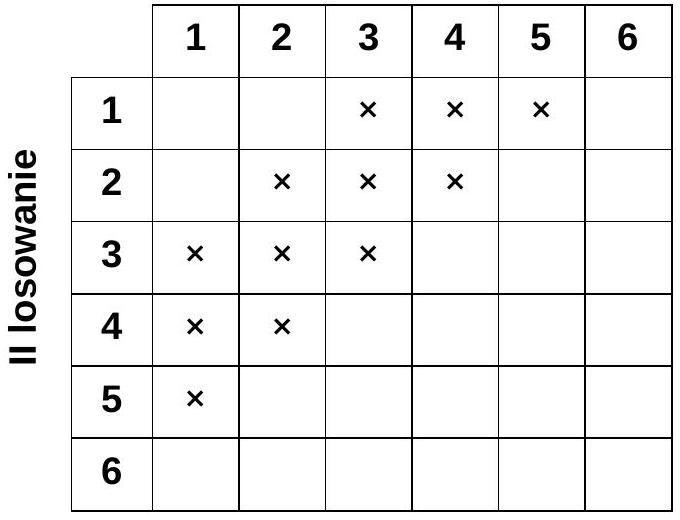
\includegraphics[max width=\textwidth, center]{2025_02_07_6828143ce1e2fe8e0865g-24}

Symbolem × oznaczono zdarzenia elementarne sprzyjające zdarzeniu $A$.\\
Wszystkich zdarzeń elementarnych w tym doświadczeniu jest 36.\\
Wszystkich zdarzeń elementarnych sprzyjających zdarzeniu $A$ jest 12.\\
Stąd $P(A)=\frac{|A|}{|\Omega|}=\frac{12}{36}=\frac{1}{3}$.

Sposób 3. (drzewo stochastyczne)\\
Rysujemy drzewo stochastyczne rozważanego doświadczenia.\\
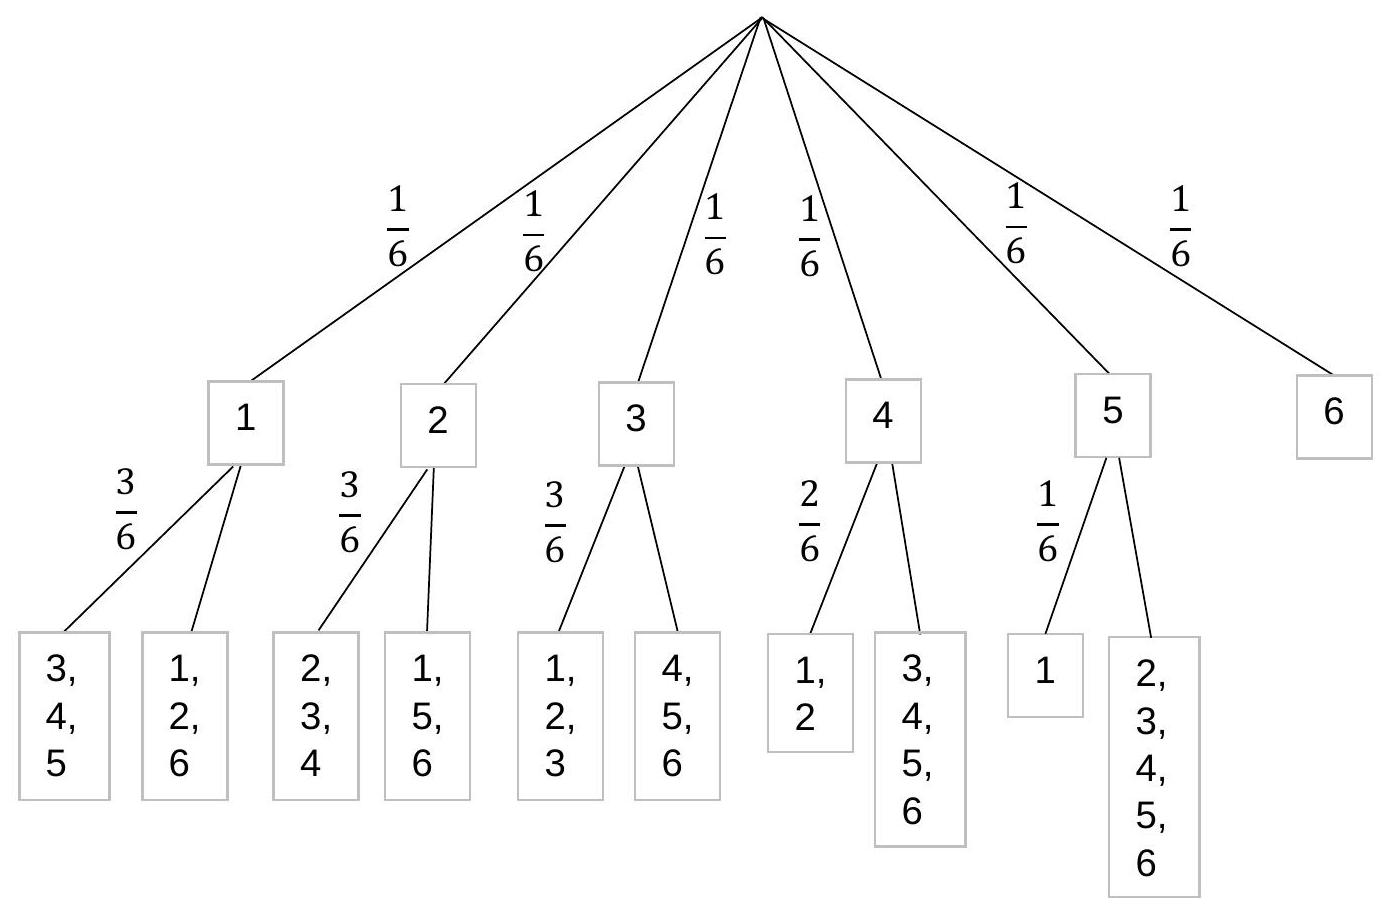
\includegraphics[max width=\textwidth, center]{2025_02_07_6828143ce1e2fe8e0865g-25}

Prawdopodobieństwo zdarzenia $A$ jest równe

$$
P(A)=\frac{1}{6} \cdot \frac{3}{6}+\frac{1}{6} \cdot \frac{3}{6}+\frac{1}{6} \cdot \frac{3}{6}+\frac{1}{6} \cdot \frac{2}{6}+\frac{1}{6} \cdot \frac{1}{6}=\frac{12}{36}=\frac{1}{3}
$$

Zadanie 35. (0-5)

\begin{center}
\begin{tabular}{|l|l|}
\hline
\multicolumn{2}{|c|}{Wymagania egzaminacyjne 2021} \\
\hline
\multicolumn{1}{|c|}{Wymaganie ogólne} & \multicolumn{1}{c|}{Wymagania szczegółowe} \\
\hline
IV. Użycie i tworzenie strategii. & Zdający: \\
 & 8.1) wyznacza równanie prostej \\
 & przechodzącej przez dane dwa punkty \\
 & (w postaci kierunkowej lub ogólnej); \\
 & 8.3) wyznacza równanie prostej, która jest \\
 & równoległa lub prostopadła do prostej \\
 & danej w postaci kierunkowej i przechodzi \\
 & przez dany punkt; \\
 & 8.4) oblicza współrzędne punktu przecięcia \\
 & dwóch prostych; \\
 & 8.6) oblicza odległość dwóch punktów. \\
\hline
\end{tabular}
\end{center}

\section*{Zasady oceniania}
\section*{Zdający otrzymuje}
 1 p. gdy:\begin{itemize}
  \item spełni jeden z poniższych warunków:
\end{itemize}

\begin{enumerate}
  \item obliczy współczynnik kierunkowy równania prostej $A B$ : $a_{A B}=-\frac{1}{3}$ lub zapisze równanie prostej $A B$ w postaci ogólnej $x+3 y-16=0$
  \item obliczy wspótrzędne środka $M$ odcinka $A B$ : $M=\left(-\frac{13}{2}, \frac{15}{2}\right)$
  \item przyjmie pierwszą współrzędną punktu $C$ równą zeru i zapisze np. $C=\left(0, y_{C}\right)$
  \item zapisze równość $\quad|A C|=|B C|$ w zależności od współrzędnych punktu $C=\left(x_{C}, y_{C}\right), \mathrm{np}$.:
\end{enumerate}

$$
\sqrt{\left(x_{C}-(-20)\right)^{2}+\left(y_{C}-12\right)^{2}}=\sqrt{\left(x_{C}-7\right)^{2}+\left(y_{C}-3\right)^{2}}
$$

ALBO

\begin{itemize}
  \item zastosuje poprawną metodę obliczenia długości boku $A B$ trójkąta i uzyska poprawny wynik: $|A B|=9 \sqrt{10}$
\end{itemize}

Zdający otrzymuje\\
gdy:

\begin{itemize}
  \item spełni jeden $z$ warunków 1)-4) określonych w punktorze pierwszym zasad oceniania za 1 punkt oraz obliczy długość boku $A B$ trójkąta\\
ALBO
  \item spełni jeden z poniższych warunków:
\end{itemize}

\begin{enumerate}
  \item zapisze równanie symetralnej $k$ odcinka $A B: y-\frac{15}{2}=3\left(x+\frac{13}{2}\right) \quad$ lub $y=3 x+27$
  \item zapisze równanie, w którym niewiadomą jest druga współrzędna wierzchołka $C$, wynikające z prostopadłości odpowiednich wektorów, np. $\overrightarrow{M A}$ oraz $\overrightarrow{M C}$ :
\end{enumerate}

$$
-\frac{27}{2} \cdot \frac{13}{2}+\frac{9}{2} \cdot\left(y_{C}-\frac{15}{2}\right)=0
$$

\begin{enumerate}
  \setcounter{enumi}{2}
  \item zapisze układ równań $z$ dwiema niewiadomymi, np.:
\end{enumerate}

$$
\sqrt{\left(x_{C}-(-20)\right)^{2}+\left(y_{C}-12\right)^{2}}=\sqrt{\left(x_{C}-7\right)^{2}+\left(y_{C}-3\right)^{2}} \text { i } x_{C}=0
$$

\section*{Zdający otrzymuje}
gdy:

\begin{itemize}
  \item spełni jeden z warunków 1)-3) określonych w punktorze drugim zasad oceniania za 2 punkty oraz obliczy długość boku $A B$ trójkąta\\
ALBO
  \item zastosuje poprawną metodę obliczenia drugiej współrzędnej punktu $C$ i obliczy współrzędne punktu: $C=(0,27)$
\end{itemize}

\section*{Zdajacy otrzymuje}
4 p.\\
gdy zastosuje poprawną metodę obliczenia drugiej współrzędnej punktu $C$ oraz poprawną metodę obliczenia jednego z boków trójkąta $A B C$ i uzyska poprawne wyniki: $C=(0,27)$ oraz $|A B|=9 \sqrt{10}$ (lub $|B C|=25$ ).

\section*{Zdający otrzymuje}
5 p. gdy zastosuje poprawną metodę wyznaczenia współrzędnych punktu $C$ oraz obliczy obwód $L$ trójkąta $A B C$ i uzyska poprawne wyniki: $L=9 \sqrt{10}+50, C=(0,27)$.

\section*{Uwagi:}
\begin{enumerate}
  \item Jeżeli zdający rozważa punkt $C$ leżący na osi $O y$ i w rozwiązaniu popełnia tylko błędy rachunkowe, które nie przekreślają poprawności rozumowania, to za całe rozwiązanie może otrzymać co najwyżej 4 punkty.
  \item Jeżeli zdający przyjmie błędnie, że wierzchołek $C$ leży poza osią $O y$ i korzysta z tego w rozwiązaniu, to może otrzymać za całe rozwiązanie co najwyżej 3 punkty.
  \item Rozwiązania odczytywane.\\
a) Jeżeli zdający wyznacza współrzędne punktu $C$, wykorzystując punkty kratowe: zaznaczy w układzie współrzędnych poprawnie punkty $A$ i $B$, narysuje trójkąt równoramienny $A B C$, a punkt $(0,27)$ oznaczy przez $C$, to za wyznaczenie współrzędnych punktu $C$ może uzyskać 3 punkty.\\
b) Jeżeli zdający rysuje w układzie współrzędnych symetralną odcinka $A B$ i odczytuje współrzędne punktu $C$ i zapisuje $C=(0,27)$ oraz sprawdzi rachunkowo, że $|A C|=|B C|$, to za tę część rozwiązania otrzymuje 3 punkty (jeżeli tego sprawdzenia nie wykona, to otrzymuje za tę część rozwiązania 2 punkty, a gdy odczyta błędne współrzędne punktu $C$, to otrzymuje $\mathbf{0}$ punktów).
  \item Jeżeli zdający rozważa dwa różne położenia punktu $C$ i nie odrzuca niewłaściwego rozwiązania, to otrzymuje co najwyżej 4 punkty.
  \item Jeżeli zdający nie sporządzi rysunku i zapisze tylko $C=(0,27)$, to otrzymuje $\mathbf{0}$ punktów; jeżeli zdający nie sporządzi rysunku, lecz zapisze $C=(0,27)$ i dalej kontynuuje rozwiązanie, to może otrzymać co najwyżej 2 punkty.
  \item Jeżeli zdający popełni błąd merytoryczny, to może otrzymać co najwyżej 3 punkty.
\end{enumerate}

\section*{Przykładowe pełne rozwiązania}
\section*{Sposób 1.}
Obliczamy współczynnik kierunkowy prostej $A B$ :

$$
a_{A B}=\frac{3-12}{7-(-20)}=-\frac{9}{27}=-\frac{1}{3}
$$

Zatem współczynnik kierunkowy symetralnej $k$ odcinka $A B$ jest równy

$$
a_{k}=3
$$

Symetralna $k$ przechodzi przez środek $M$ odcinka $A B$. Obliczamy współrzędne punktu $M$ :

$$
M=\left(\frac{-20+7}{2}, \frac{12+3}{2}\right)=\left(-\frac{13}{2}, \frac{15}{2}\right)
$$

Zatem prosta $k$ ma równanie postaci

$$
\begin{gathered}
y-\frac{15}{2}=3\left(x-\left(-\frac{13}{2}\right)\right) \\
y-\frac{15}{2}=3 x+\frac{39}{2} \\
y=3 x+27
\end{gathered}
$$

Ponieważ punkt $C$ leży na osi $O y$ i na prostej $k$, więc współrzędne punktu $C$ są równe $C=(0,27)$.\\
Obliczamy długości boków trójkąta:

$$
\begin{aligned}
& |A C|=\sqrt{(0-(-20))^{2}+(27-12)^{2}}=\sqrt{400+225}=\sqrt{625}=25 \\
& |A B|=\sqrt{(7-(-20))^{2}+(3-12)^{2}}=\sqrt{729+81}=\sqrt{810}=9 \sqrt{10}
\end{aligned}
$$

Obliczamy obwód $L$ trójkąta $A B C$ :

$$
L=|A B|+|B C|+|C A|=9 \sqrt{10}+25+25=50+9 \sqrt{10}
$$

\section*{Sposób 2.}
Ponieważ wierzchołek $C$ trójkąta równoramiennego $A B C$ leży na osi $O y$, więc jego współrzędne są równe $C=\left(0, y_{C}\right)$.

Ponieważ $|A C|=|B C|$, więc $|A C|^{2}=|B C|^{2}$. Stąd i ze wzoru na odległość między dwoma punktami otrzymujemy równanie

$$
(0-(-20))^{2}+\left(y_{C}-12\right)^{2}=(0-7)^{2}+\left(y_{C}-3\right)^{2}
$$

$$
\begin{gathered}
400+y_{C}^{2}-24 y_{C}+144=49+y_{C}^{2}-6 y_{C}+9 \\
-18 y_{C}=-486 \\
y_{C}=27
\end{gathered}
$$

Zatem $C=(0,27)$.\\
Obliczamy długości boków trójkąta:

$$
\begin{aligned}
& |A C|=\sqrt{(0-(-20))^{2}+(27-12)^{2}}=\sqrt{400+225}=\sqrt{625}=25 \\
& |A B|=\sqrt{(7-(-20))^{2}+(3-12)^{2}}=\sqrt{729+81}=\sqrt{810}=9 \sqrt{10}
\end{aligned}
$$

Obliczamy obwód $L$ trójkąta $A B C$ :

$$
L=|A B|+|B C|+|C A|=9 \sqrt{10}+25+25=50+9 \sqrt{10}
$$

\section*{Sposób 3.}
Niech $y$ oznacza drugą współrzędną wierzchołka $C$, tj. $C=(0, y)$.\\
Obliczamy wspórzędne środka $M$ odcinka $A B$ :

$$
M=\left(\frac{-20+7}{2}, \frac{12+3}{2}\right)=\left(-\frac{13}{2}, \frac{15}{2}\right)
$$

Obliczamy współrzędne wektorów $\overrightarrow{M A}$ oraz $\overrightarrow{M C}$ :

$$
\begin{aligned}
& \overrightarrow{M A}=\left[-20+\frac{13}{2}, 12-\frac{15}{2}\right]=\left[-\frac{27}{2}, \frac{9}{2}\right] \\
& \overrightarrow{M C}=\left[0+\frac{13}{2}, y-\frac{15}{2}\right]=\left[\frac{13}{2}, y-\frac{15}{2}\right]
\end{aligned}
$$

Wektor $\overrightarrow{M A}$ jest prostopadły do wektora $\overrightarrow{M C}$, zatem

$$
\begin{gathered}
-\frac{27}{2} \cdot \frac{13}{2}+\frac{9}{2} \cdot\left(y-\frac{15}{2}\right)=0 \\
\frac{9}{2} y=\frac{486}{4} \\
y=27
\end{gathered}
$$

Zatem punkt $C$ ma współrzędne $C=(0,27)$.\\
Obliczamy długości boków trójkąta $A B C$ :

$$
\begin{aligned}
& |A C|=\sqrt{(0-(-20))^{2}+(27-12)^{2}}=\sqrt{400+225}=\sqrt{625}=25 \\
& |A B|=\sqrt{(7-(-20))^{2}+(3-12)^{2}}=\sqrt{729+81}=\sqrt{810}=9 \sqrt{10}
\end{aligned}
$$

Egzamin maturalny z matematyki (poziom podstawowy) - termin główny 2021 r.

Obliczamy obwód $L$ trójkąta $A B C$ :

$$
L=|A B|+|B C|+|C A|=9 \sqrt{10}+25+25=50+9 \sqrt{10}
$$

\section*{Ocena prac osób ze stwierdzona dyskalkulia}
Obowiązują zasady oceniania stosowane przy sprawdzaniu prac zdających bez stwierdzonej dyskalkulii z dodatkowym uwzględnieniem:\\
I. ogólnych zasad oceniania zadań otwartych w przypadku arkuszy osób ze stwierdzoną dyskalkulią (punkty 1.-12.);\\
II. dodatkowych szczegółowych zasad oceniania zadań otwartych w przypadku arkuszy osób ze stwierdzoną dyskalkulią - matura z matematyki, poziom podstawowy, termin główny 2021.\\
I. Ogólne zasady oceniania zadań otwartych w przypadku arkuszy osób ze stwierdzona dyskalkulia

\begin{enumerate}
  \item Nie należy traktować jako błędy merytoryczne pomyłek, wynikających z:
\end{enumerate}

\begin{itemize}
  \item błędnego przepisania,
  \item przestawienia cyfr,
  \item zapisania innej cyfry, ale o podobnym wyglądzie,
  \item przestawienia położenia przecinka.
\end{itemize}

\begin{enumerate}
  \setcounter{enumi}{1}
  \item W przypadku błędów, wynikających ze zmiany znaku liczby, należy w każdym zadaniu oddzielnie przeanalizować, czy zdający opanował inne umiejętności, poza umiejętnościami rachunkowymi, oceniane w zadaniu. W przypadku opanowania badanych umiejętności zdający powinien otrzymać przynajmniej 1 punkt.
  \item We wszystkich zadaniach otwartych, w których wskazano poprawną metodę rozwiązania, części lub całości zadania, zdającemu należy przyznać przynajmniej 1 punkt, zgodnie z kryteriami do poszczególnych zadań.
  \item Jeśli zdający przedstawia nieprecyzyjne zapisy, na przykład pomija nawiasy lub zapisuje nawiasy w niewłaściwych miejscach, ale przeprowadza poprawne rozumowanie lub stosuje właściwą strategię, to może otrzymać przynajmniej 1 punkt za rozwiązanie zadania.
  \item W przypadku zadania wymagającego wyznaczenia pierwiastków trójmianu kwadratowego zdający może otrzymać 1 punkt, jeżeli przedstawi poprawną metodę wyznaczania pierwiastków trójmianu kwadratowego, przy podanych w treści zadania wartościach liczbowych.
  \item W przypadku zadania wymagającego rozwiązania nierówności kwadratowej zdający może otrzymać 1 punkt, jeżeli stosuje poprawny algorytm rozwiązywania nierówności kwadratowej, przy podanych w treści zadania wartościach liczbowych.
  \item W przypadku zadania wymagającego stosowania własności funkcji kwadratowej zdający może otrzymać 1 punkt za wykorzystanie konkretnych własności funkcji kwadratowej, istotnych przy poszukiwaniu rozwiązania.
  \item W przypadku zadania wymagającego zastosowania własności ciągów arytmetycznych lub geometrycznych zdający może otrzymać 1 punkt, jeżeli przedstawi wykorzystanie takiej własności ciągu, która umożliwia znalezienie rozwiązania zadania.
  \item W przypadku zadania wymagającego analizowania figur geometrycznych na płaszczyźnie kartezjańskiej zdający może otrzymać punkty, jeżeli przy poszukiwaniu rozwiązania przedstawi poprawne rozumowanie, wykorzystujące własności figur geometrycznych lub zapisze zależności, pozwalające rozwiązać zadanie.
  \item W przypadku zadania z rachunku prawdopodobieństwa zdający może otrzymać przynajmniej 1 punkt, jeśli przy wyznaczaniu liczby zdarzeń elementarnych\\
sprzyjających rozważanemu zdarzeniu przyjmuje określoną regularność lub podaje prawidłową metodę wyznaczenia tej liczby zdarzeń elementarnych.
  \item W przypadku zadania z geometrii zdający może otrzymać przynajmniej 1 punkt, jeżeli podaje poprawną metodę wyznaczenia długości odcinka potrzebnej do znalezienia rozwiązania.
  \item W przypadku zadania wymagającego przeprowadzenia dowodu (z zakresu algebry lub geometrii), jeśli w przedstawionym rozwiązaniu zdający powoła się na własność, która wyznacza istotny postęp, prowadzący do przeprowadzenia dowodu, to może otrzymać 1 punkt.
\end{enumerate}

\section*{II. Dodatkowe szczegółowe zasady oceniania zadań otwartych w przypadku arkuszy osób ze stwierdzona dyskalkulia}
\section*{Zadanie 29.}
\section*{Zdający otrzymuje 1 pkt, jeżeli:}
\begin{itemize}
  \item stosuje poprawną metodę obliczenia pierwiastków trójmianu kwadratowego $x^{2}-5 x-14$, tzn. stosuje wzory na pierwiastki trójmianu kwadratowego i oblicza te pierwiastki, popełniając błędy o charakterze dyskalkulicznym\\
ALBO
  \item zdający w wyniku obliczeń otrzyma wyróżnik ujemny, ale konsekwentnie narysuje parabolę ALBO
  \item Poprawnie rozwiąże nierówność $x^{2}-5 x \leq 0$.
\end{itemize}

\section*{Zdający otrzymuje 2 pkt, jeżeli:}
\begin{itemize}
  \item pomyli porządek liczb na osi liczbowej, np. zapisze zbiór rozwiązań nierówności w postaci $x \in[7,-2]$.
\end{itemize}

\section*{Uwaga:}
\begin{enumerate}
  \item Jeżeli zdający zapisze zbiór rozwiązań nierówności w postaci przedziału otwartego, to może otrzymać co najwyżej 1 pkt.
\end{enumerate}

\section*{Zadanie 30.}
\section*{Zdający otrzymuje 1 pkt, jeżeli:}
przekształci nierówność $\frac{a}{b}<\frac{a+c}{b+c}$ do postaci $\frac{a(b+c)}{b}<a+c$ lub $a<\frac{b(a+c)}{b+c}$.

\section*{Zadanie 31.}
Stosuje się zasady oceniania arkusza standardowego.

\section*{Zadanie 32.}
\section*{Zdający otrzymuje 1 pkt, jeżeli:}
\begin{itemize}
  \item popełnia błąd przy przekształceniu równania $\frac{3 x+2}{3 x-2}=4-x$ do postaci równania kwadratowego, lecz dalej stosuje poprawną metodę rozwiązania otrzymanego równania i konsekwentnie oblicza pierwiastki tego równania.
\end{itemize}

\section*{Zadanie 33.}
\section*{Zdający otrzymuje 1 pkt, jeżeli:}
\begin{itemize}
  \item zastosuje poprawną metodę obliczenia długości boku trójkąta $A B C$ (stosuje wzór na pole trójkąta równobocznego)\\
ALBO
  \item zapisze, że $\frac{P_{A B C}}{P_{A K L}}=\left(\frac{3}{2}\right)^{2}$.
\end{itemize}

\section*{Zdający otrzymuje 2 pkt, jeżeli:}
\begin{itemize}
  \item zastosuje poprawną metodę wyznaczenia długości boku trójkąta $A K L$, popełnia jeden błąd o charakterze dyskalkulicznym i konsekwentnie doprowadza rozwiązanie do końca.
\end{itemize}

\section*{Uwaga:}
W ocenie rozwiązania zadania 33. (dla zdających z dyskalkulią) nie stosuje się uwagi nr 2 ze standardowych zasad oceniania.

\section*{Zadanie 34.}
\section*{Zdający otrzymuje 1 pkt, jeżeli:}
\begin{itemize}
  \item zapisze jedynie liczbę 36 (należy traktować to jako wyznaczenie liczby wszystkich zdarzeń elementarnych).\\
ALBO
  \item zapisze liczbę 12, o ile z zapisów wynika, że interpretuje tę liczbę jako liczbę zdarzeń elementarnych sprzyjających zdarzeniu $A$ (np. jest to zilustrowane wypisaniem kilku zdarzeń elementarnych sprzyjających zdarzeniu $A$ i zdający nie zapisze zdarzeń elementarnych, które nie sprzyjają zdarzeniu $A$ ).
\end{itemize}

\section*{Zdający otrzymuje 2 pkt, jeżeli:}
\begin{itemize}
  \item poprawnie wypisze (lub zaznaczy) wszystkie zdarzenia elementarne sprzyjające zdarzeniu $A$, popełni błąd w ich zliczeniu i konsekwentnie zapisze wynik $\frac{x}{36}$, gdzie $x$ jest liczbą zliczonych zdarzeń elementarnych sprzyjających zdarzeniu $A$.
\end{itemize}

\section*{Uwaga:}
W ocenie rozwiązania zadania 34. (dla zdających z dyskalkulią) nie stosuje się uwagi nr 1 ze standardowych zasad oceniania.

\section*{Zadanie 35.}
\section*{Zdający otrzymuje 1 pkt, jeżeli:}
\begin{itemize}
  \item zastosuje poprawną metodę obliczenia długości boku $A B$ trójkąta
\end{itemize}

\section*{ALBO}
\begin{itemize}
  \item zastosuje poprawną metodę obliczenia współczynnika kierunkowego równania prostej $A B$
\end{itemize}

\section*{Zdający otrzymuje 2 pkt, jeżeli:}
\begin{itemize}
  \item zastosuje poprawną metodę wyznaczenia równania symetralnej odcinka $A B$
\end{itemize}

\section*{ALBO}
\begin{itemize}
  \item stosuje poprawne metody wyznaczenia wielkości w punktach 1)-4) pierwszego punktora standardowych zasad oceniania za 1 pkt oraz zastosuje poprawną metodę obliczenia długości boku $A B$ trójkąta.
\end{itemize}


\end{document}